\documentclass{article}
\usepackage[utf8]{inputenc}
\title{Lecture 8 mutliclass classification }
\author{wbg231 }
\date{December 2022}
\newcommand{\R}{$\mathbb{R}$}
\newcommand{\B}{$\beta$}
\newcommand{\A}{$\alpha$}
\newcommand{\D}{\Delta}

\newcommand{\avector}[2]{(#1_2,\ldots,#1_{#2})}
\newcommand{\makedef}[2]{$\textbf{#1}$:#2 }
\usepackage{tikz,graphicx,hyperref,amsmath,amsfonts,amscd,amssymb,bm,cite,epsfig,epsf,url}

\begin{document}

\maketitle

\section{motivation}
\begin{itemize}
\item up to this point we have only done binary classification
\item binary classification works well for a lot of problems (spam vs non spam) or (positive vs negative sentiment )
\item but that does not deal with all types of questions, like maybe we want to recognize the objects
in a photograph, or face recognition or recognizing letters from handwriting  (some of these questions
have 1000's or millions of classes)
\item what are some potential issues with many classes? 
\begin{enumerate}
    \item computation cost (may have to train many classification models)
    \item class imbalance (if we are training a classifier to detect dog or not dog there are likely many more examples of not dog than dog )
    \item different cost of errors (want to be sure it is a dog, versus most of the time it is not a dog. that is if we are training a one versus all classifier we want to only predict positive when we are really confident in our guess )
\end{enumerate}
\subsection*{plan for today}
\item today we are going to explore the following questions
\item how to reduce mutliclass classification into binary classification. 
\item we could train many binary classifiers, (could also do a linear regression and bin your regression outputs to a certain class like if $f(x)\in [0,1)$ say it is a dog if $f(x)\in [1,2)$ say it is a cat. this is kind of an arbitrary way to do it though. ) 
\item how do generalize what we learned in binary classification to mutliclass classification (we can think about loss functions)
\item we are also going to talk about structured prediction
\section{reduction to binary classification}
\subsection*{one vs all and one vs rest }
\item suppose we have an input space $X$ (general)
\item and outputs space is discrete integers $Y=\{1...k\}:\forall y_i\in \mathbb{Z}$
\item we are going to train k binary classifiers once for each class $h_1...h_k:X\rightarrow \mathbb{R}$ (map from input space to real numbers)
\item classifier $h_i$ distinguishes class i from all other classes (that is $h_i(x)=1\Rightarrow \text{ we think x is class i } $ and $h_i(x)=-1\Rightarrow \text{ we think x is not class i } $
\item this is what we call the one versus all (or one versus rest)
\item we predict by a \textbf{majority vote } such that $$h(x)=argmax_{i\in [1,k]}h_i(x)$$
\item and we break ties arbitrarily 
\subsection*{example}
\item suppose we have a dataset with 3 classes that looks like this \\
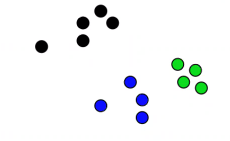
\includegraphics[width=5cm]{lecture_notes/lecture_8/immages/l8_1.png}
\item the output of our model should be 1,2,3 for any given x 
\item we can train 1 versus all classifiers (here we are assuming only linear classifiers) but in theory it does not matter if they are linear or not. 
\\ 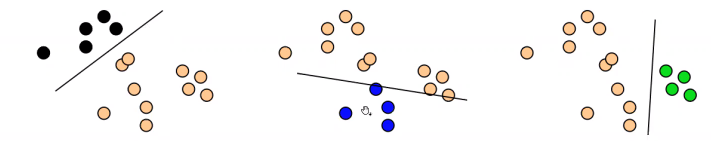
\includegraphics[width=5cm]{lecture_notes/lecture_8/immages/l8_2.png}
\item so we trained the following three classifiers with the following 3 decision boundaries 
\item here we are assuming that each set is linearly separable from the rest. 
\item in the ideal case only one of the classes should have a positive score and the others should have negative values
\item there are cases where we can not linearly separate the data. 
\item and so one versus all (with a linear assumption ) will not work here. 
\\ 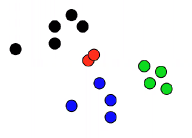
\includegraphics[width=5cm]{lecture_notes/lecture_8/immages/l8_3.png}
\item such as here 
\subsection*{all versus all, one vs one or all pairs}
\item as we showed above the one versus all does not work in all cases, such as when as the cases where the classes can not be serrated 
\item another way to deal with this is the all versus all classifier (also called one vs one or all pairs )

\item suppose we have an input space $X$ (general)
\item and outputs space is discrete integers $Y=\{1...k\}:\forall y_i\in \mathbb{Z}$
\item we are going to train $\begin{pmatrix}k\\2
\end{pmatrix}$ (that is the number of permutations of length 2 ie all pairs of classes) where $h_{i,j}:X\rightarrow \mathbb{R} $  where $where i\in [1,k], j[i+1,k]$
\item  $h_i(x)=1\Rightarrow \text{ we think x is class i } $ and $h_i(x)=-1\Rightarrow \text{ we think x is class j } $  
\item we again predict using a majority vote such that 
$$h(x)=argmax_{i\in [1,k]}\Sigma_{i\neq j}h_{i,j}(x)\mathbb{I}(i<j)+h_{j,i}(x)\mathbb{I}(j<i)
$$ 
so each class gets (k-1) votes for the k-1 classifiers that take value positive one if we think it is that class so at most you can get each class gets at most $k-1$ 
\item again ties can be broken in an arbitrary way. 
\item note that as we are training $\begin{pmatrix}k\\2
\end{pmatrix}$ classifiers our number of classifiers will quadratically increase with the number of classes 
\item in general the classifiers will not be calibrated so we will just sum up the integer number of votes
\subsection*{Example}
\item suppose we again have this data set 
 \\ 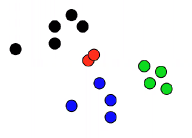
\includegraphics[width=5cm]{lecture_notes/lecture_8/immages/l8_3.png}
\item here we are assuming that each pair of classes is linearly separable this is more expressive than one versus all.
\item   so here we are training $\begin{pmatrix}4\\2
\end{pmatrix}=6$ classifiers 
\item this does septate the classes 
\subsection*{one vs all vs all vs all}
\item here is a chart comparing on versus all and all versus all 
\\  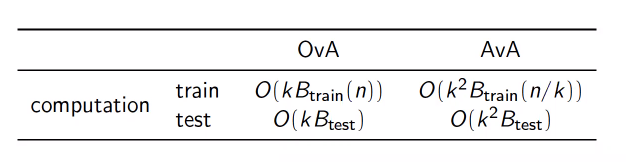
\includegraphics[width=5cm]{lecture_notes/lecture_8/immages/l8_4.png}
\item here we are assuming that each pair of classes is linearly separable this is more expressive than one versus all.
\item all vs all requires a quadratic number of classifiers while one vs all only requires a linear number of classifiers
\item so when we are training a one vs all classifier we need to train each classifier on our total number of data points (that is all training data marked for every class)
\item in contrast when we are training are all vs all classifier each classifier is only concerned with the data that deals with its one of two classes which in big O notation is $\frac{n}{k}$ (the point is you are dealing with a much smaller dataset for each of the small classifiers) (this also assumes that the dataset is balanced)
\item in terms of test time there is not really a difference as in either case we are taking one example and running through all classifiers we have 
\item there are some challenges with this 
\begin{enumerate}
    \item while training a one vs all classifier if the data is imbalanced if you have 10 classes and 100 data points that are evenly distributed across all classes. for each 1 vs all classifier you will have 10 positive examples and 90 negative examples meaning we will have large calibration issues
    \item all versus all while training has a small training set for each classifier (if again we have 100 data points that are evenly distributed across all classes then for each classifier we have 10 positive examples and 10 negative examples to train each classifier on )
    \item so calibration (ie how we compare the real value output from our classifiers) is an issue  (do we scale one class up or down)?  is an issue for both models
    \item tie breaking is also arbitrary which is not great 
\end{enumerate}
\item so these are simple models, but they lack theoretical rigor. 
\item they do work well in practice though 
\subsection*{code words for labels}
\item the basic idea here is we can encode labels as binary codes  and predict the code bits directly 
\item this allows us to train fewer binary classifiers to do the same task. 
\item so suppose we want to do one versus all classification  with 4 classes and 4 classifiers 
\item  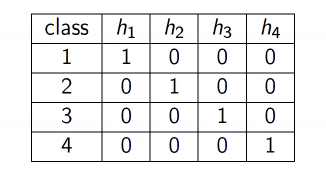
\includegraphics[width=5cm]{lecture_notes/lecture_8/immages/l8_5.png}
\item here we are one hot encoding our labels, here each class gets one representation 
\item ideally there are only 4 situations that can happen. each of the class labels
\item but in practice if we train our classifiers independently  it is possible for us to get results that do not neatly fit into any class  (like 1100)
\item it is hard to predict using that. 
\item so this encoding uses k bits for k classes, can we reduce the number of bits we are using? yes given k bits there are $2^k$ total number of codes 
\item one versus all uses k bits to represent k classes. there are $2^k$ possible encodings done with k bits
\subsection*{error correcting output codes (ECOC) }
\item in general you can use between log(k) and k bits to represent k classes
\item here is an example where we use 6 bits  to represent 8 classes. 
 \item  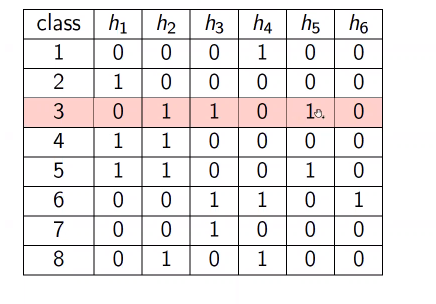
\includegraphics[width=5cm]{lecture_notes/lecture_8/immages/l8_6.png}
\item so for instance class 3 is coded as $011011$
\item so in this context we train one classifiers $h_i$ for each bit (so in the example 6) and classifier $h_i$ takes value 1 when the i-th bit is 1, and $-1$ when the ith bit is zero
\item we then predict classes based on the closest label in terms of hamming distance ie we take the label which would require the minimum bit changes to get. that is in this case basically how many bits different
\item also note that all of our classifier's are independent in this case.   
\item so if we have log(k) bits then every possible combination of bits will be matched to a class exactly so we will not have to worry about hamming distance 
\item there is a problem of code design we want good binary classifiers, we may want our independent bits to represent something that can go do down a decision tree so that each classifier knows what it it does. 
\item this type of approach is called error correcting output codes. so even if we make a mistake and predict a class that does not exist we could correct, it using hamming distance 
\item this approach is computationally efferent we only need to use between log(k) and k bits. 
\item why not always use the minimal number of bits 
\begin{enumerate}
    \item if the minimum hamming distance between any pair of codes words is d, then this algorithm can only correct $\lfloor\frac{d-1}{2}\rfloor$ errors. 
    \item that is if code names are close to one another then we are not very robust to errors ie all classifiers need to get every bit right or else we will mislabel an example 
\end{enumerate}
\item so we want to find a ballance between using too many bits and not having enough classifiers to correct for errors
\item there are some theoretical results that could be cool looking through later on the course website
\subsection*{review}
\item so far we have discussed approaches that reduce mutliclass problems to binary classifier problems
\item the key here is to design a natural binary classification problem without using a lot of computation
\item the issues are that this does not generalize to really large numbers of classes 
\item so there are other methods we can work with 
\section{mutliclass classification loss functions}
\subsubsection*{review of binary logistic regression}
\item our goal is given an input x we want to predict an output of either zero or one. 
\item the output of our model is given by $$f(x)=sigmoid(z)=\frac{1}{1+e^{-z}}=\frac{1}{1+e^{-w^{t}x-b}}$$ this transforms our prediction to be between zero and one so we can interpret it as a probability
\item the given we understand that $f(x)=P(x=1)$ it is natural that $$P(x=0)=(1-P(x=1))=1-f(x)=\frac{e^{-w^tx-b}}{1+e^{-w^tx-b}}=\frac{e^{-w^tx-b}}{1+e^{-w^tx-b}}*\frac{e^{w^txb}}{e^{w^txb}}=$$ $$\frac{1}{1+e^{w^tx-n}}=sigmoid(-z)=f(-x)$$
\item another way to think of this is that to train for one class (1) we are Learning parameters w,b and to train for the zero class we are learning parameters -w,-b
\item so in binary logistic regression even if we are only training with one set of parameters we are implicitly learning another which is just fully determined by the first set
\subsection*{mutliclass logistic regression}
\item now what is we have one $w_c$ for each class c
\item we can define a  more general type of sigmoid function also called the soft max function as $$f_{c}(c)=\frac{e^{w_{c}^tx+b_c}}{\Sigma_{c}e^{w_{c}^tx+b_c}}$$
\item the idea is that this score sums up to 1, but every classes is represented by a non-normalized score $e^{w_c^t+b_c}$
\item loss function $L=\Sigma_{i}-y_c^ilog(f_c(x^i))$ 
\item this is a more generalized form of the binary case. 
\item they write that $\frac{\partial L}{\partial z}=f-y$ and say z is the sigmoid function but i am not sure what they are trying to say here
\subsection*{comparison to one versus all}
\item for both one vs all and logistic regression all the following holds
\item the hypothesis space for k classes here is $$\mathcal{F}=\{x\rightarrow h_i(x)|h_1...h_k\in \mathcal{H}\}$$ that is we are trinaing 
k independent classifiers which will all be in the single hypothesis $\mathcal{H}=\{h:X\rightarrow\mathbb{R}\}$ that is maps from our input space to real numbers 
\item $h_i(x)$ scores how likely we think it is that input x is from class i 
\item they just more or less use different score functions
\item for one versus all objective $h_i(x)>0$ for all x of label i and $h_i(x)<0$ for all other labels
\item we predict at test time to predict (x,i) correctly we just need $h_{i}(x)>h_{j}(x)\forall j\neq i$
\section*{multiclass perceptron }
\item for the perceptron model the base linear predictor is given by $h_(x)=w_i^{t}x:w\in \mathbb{R}^{d}$
\item and the algorithm is 
\begin{enumerate}
    \item given a mutliclass dataset $\mathcal{D}=\{x,y\}$ so note that this means for each of the k predictors we are learning d weights so we will in total have a weight matrix $W\in \mathbb{R}^{k \times d }$
    \item initialize $w\leftarrow 0$
    \item for iter=1,2...T do
    \begin{enumerate}
        \item for $(x,y)\in \mathcal{D}$
        \begin{enumerate}
        \item $\hat{y}=argmax_{y'\in y}w^t_{y'}x$ highest scoring class (ie class we are most confident it is )
        \item if $\hat{y}\neq y$ then we have made a mistake  
        \begin{enumerate}
            \item $w_{y}\leftarrow w_y+x$ move wights of true class closer to input x  
            \item $w_{\hat{y}}\leftarrow w_{\hat{y}}-x$ move the wrong class wights further from x.
        \end{enumerate}
        \item end 
    \end{enumerate}
    \item end 
    \end{enumerate}
    \item end 
\end{enumerate}
\item for each class we have a base linear predictor this is pretty similar to the softmax base in that it is an inner product
\item this is very similar to the original perceptron algorithm
\item now for each class we have a 
\subsection*{rewriting the scoring function}
\item we want to be able to scale to many classes 
\item so if we have $W=k\times d$ wights we may have scalability issues 
\item we want to encode the information form $W$ in a single weight vector $w\in \mathbb{R}^{d}$
\item we do this by instead of having k classifiers have one classifiers with a larger input dimension
$$w_{i}^{t}x=w^{t}\psi(x,i)$$
$$h_{i}(x)=h(x,i) $$
\item so here we are encoding are labels in the feature space using a feature transform $\psi:X\times I\rightarrow \mathbb{R}$
\item so $\psi$ represents what we call a compatibility score so it takes in pairs of labels and inputs and outputs how compatible that input and label are. 
\subsection*{the multi vector construction}
\item so given we have a weight vector $W\in \mathbb{R}^{k\times d}$ we can flatten it into a vector $w=\begin{pmatrix}
    w_{1,1} & ... & w_{1,d} &w_{2,1} &... & ... w_{k,d}
\end{pmatrix}\in \mathbb{R}^{1\times (d* k)}$ that is a row vector 
\item and then we can define $\psi:(X,Y)\rightarrow \mathbb{R}^{1\times (D * k)}$
\item then we have $<w,\psi(x,y)>=<wy,x>$
\item this allows us to re-write the mutliclass perceptron as follows

\begin{enumerate}
    \item given a mutliclass dataset $\mathcal{D}=\{x,y\}$ so note that this means for each of the k predictors we are learning d weights so we will in total have a weight matrix $W\in \mathbb{R}^{k \times d }$
    \item initialize $w\leftarrow 0$
    \item for iter=1,2...T do
    \begin{enumerate}
        \item for $(x,y)\in \mathcal{D}$
        \begin{enumerate}
        \item $\hat{y}=argmax_{y'\in y}w^t\phi({x,y'})$ highest scoring class (ie class we are most confident it is )
        \item if $\hat{y}\neq y$ then we have made a mistake  
        \begin{enumerate}
            \item $w_{y}\leftarrow w_y+\phi({x,y'})$ move wights of true class closer to $\phi({x,y'})$  
            \item $w_{\hat{y}}\leftarrow w_{\hat{y}}-\phi({x,y'})$ move the wrong class wights further from $\phi({x,y'})$.
        \end{enumerate}
        \item end 
    \end{enumerate}
    \item end 
    \end{enumerate}
    \item end 
\end{enumerate}
\subsection*{part of speech tagging}
\item input space $X=\{\text{all words}\}$
\item output space $Y=\{\text{noun, verb, adj..}\}$
\item features of $x\in X:[\text{all possible words}]$
\item how to construct our feature vector?
\item could have the multi vector construction $w\in \mathbb{R}^{d\times k}$ but this does not scale well to large feature or output spaces
\item we could also directly design features for each class $$\psi(x,y)=(\psi_{1}(x,y),\psi_{2}(x,y),..\psi_{d}(x,y))$$ 
so that is we basically have each $\psi_{i}$ looking at each element of d, which upper bounds the size of our feature space to be d \\
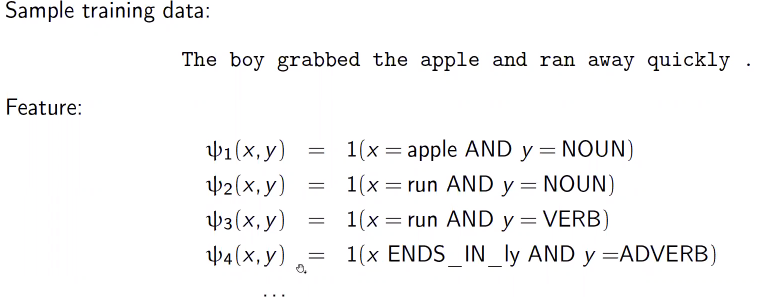
\includegraphics[width=10cm]{lecture_notes/lecture_8/immages/l8_9.png}
\item so here we have an example of our feature map capturing more fine detail about each part of the sentence than just using a one hot encoding that checks for the presence of every combination of words and part of speech
\item so what is the captured in the feature map, and when we do the dot product what are we doing (we are taking the dot product between w, $\psi(x,y)$) representing a compatibility score. 
\item so after training our $w_1..w_4$ based on our feature $\psi_{i}(x,y)$ we want the value $w_i^{t}\psi_i(x,y)$ to be large when we think having that combination of word and label is correct (so that we want  $w_1, w_3$ to be high and $w_2$ to be low)
\item keep in mind that there is no need to keep in include feature that are not in the training data as we will have no way tot rain them.
\subsection*{feature templates}
\item   maybe could take into account near by words 
\item could read of features from the training data meaning 
\item some time features could be spare 
\item could use a hash function template
\subsection*{review}
\item ingredients for mutliclass classification
\item scoring functions for each class similar to training 
\item represent labels in the input space and a single weight vector 
\item not we want to discuss generalized SVM models for multiclass classification
\section{svm}
\subsection*{why would we like svm over perceptron}
\item svm allows for non-linearity
\item svm prefers a large margin 
\item perceptron is not a maximal margin classifier it does not care as long as the classes are separated, which may not give us as much robustness 
\subsection*{margin for multiclass}
\item in the binary case the margin for $(x^{n},y^{n})$ is given by $$y^{n}f(x^{n})=y^{n}w^tx^{n}$$
\item we want our margin to be large and positive ie $w^tx^{n}$ should have the same sign as $y^n$
\item in the multiclass case we need a class specific margin for $(x^n, y^n)$ $$h(x^{n},y^{n})-h(x^n,y)$$ where $y^n$ is true class and y is the predicted label
\item that is the difference between scores of teh correct class and all other classes 
\item want the margin to be large and postive for all $y\neq y^n$
\subsection*{svm separable case}
\item in the binary classification case our linearly separable problem is $$min_{w}\frac{1}{2}||w||^{2} : y^nw^tx^n\geq 1, \forall (x^i,y^y)\in \mathbb{D}$$
\item in the multiclass case our linearity separable problem is we define our marign as $m_{n,y}(w):=<w,\psi(x^{n}, y^{n})-<w,\psi<x_n,t>$ so that is the margin of of data point n is the difference between the score of the correct class and the score of the true class 
 $$min_{w}\frac{1}{2}||w||^{2} : m_{n,y}\geq 1, \forall (x^{n}, y^{n})\in \mathbb{D}, y\neq y^{n}$$
\subsection*{hingle loss}
\item recall that hinge loss is $\ell_{hinge}(y,\hat{y})=max(0,10yh(x))$
\item and that svm can basically be thought of as optimizing hinge loss 
\item it is a convex upper bound for zero one loss
\item what's the zero one loss for mutliclass classification we can write it as $$\Delta(y,y')=\mathbb{I}(y\neq y')$$
\item so the upper bound on $\delta(y,y')$ is \\ $\hat{y}:=argmax_{y'\in y}<e,\psi(x,y')>$
\item so by that we know $<w,\psi(x,y)>\leq <w,\psi(w,\hat{y})>$ and as $y$ is the true class label we know $0\leq<w,\psi(x,y)>\leq <w,\psi(w,\hat{y})>$
\item this means we can write $\Delta(y,\hat{y})\neq \Delta(y,\hat{y})-<w,(\psi(x,y)-\psi(x,\hat{y}))>$
\item so we can define our geneal hinge loss as $$\ell_{hinge}(y,x,w):=max_{y'\in y}(\Delta (y,y')-<w,(\psi(w,y)-\psi(x,y')> )$$ where $y'$ is our predicted class and $y$ is the true class. so we are looking for the max violation effectively 
\item recall in binary svm we can write the hinge loss formulation as $$min_{w\in \mathbb{R}^{d}}\frac{1}{2}||w||^{2}+C\Sigma_{i=1}^{n}max(0,1-y^{n}w^{t}x^{n})$$
\item the multiclass objective $$min_{w\in \mathbb{R}^{d}}\frac{1}{2}||w||^{2}+C\Sigma{n=1}^{N}max_{y\in y'}(\Delta(y,y')- <x,(\psi(x,y)-\psi(x,y'))>)$$
\item so $\Delta(y,y')$ is the target margin for each class 
\item if the margin meets or exceeds $\Delta(y^n,y')\forall y\in Y$ then there is no on example n, that is there is no loss if the margin of all other classes is bellow 1 distance from the true class score than there is no loss 
\subsection*{does one versus all work in practice}
\item yeah one versus all works pretty well n practice
\item but there are a lot of mutliclass frameworks that may be better
\item all of the mutliclass frameworks preformed roughly the same 

\subsection*{mutliclass svm recap}
\item the frameworks we have developed for multiclass keeps track of compatibility features, scoring functions, multiclass margins and target margins 
\item this generalized well where k is large and only versus large is intractable. 
\item the key idea is that we can generalize across any output y by using features transforms $\psi(x,y)$
\section{introduction to structured prediction}
\subsection*{example part of speech tagging}
\item structured prediction is a big field but this is a small introduction 
\item given a sentence we may want to tag the part of speech of each word
\item so call $V=\{\text{all english words}\}$
\item call our input space $X=V^{n}$ where n is any length so that is any sequence of words
\item $P=\{\text{part of speech tags}\}$
\item $T=P^n$
\subsection*{multiclass hypothesis space}
\item so we assume that there is a discrete output space y(x), that is very large but has some structure like for instance a noun may be likely to be followed by a very or adjective but not another noun
\item our base hypothesis space (meaning the hypothesis space for a single predictor is ) $H=\{h:X\times Y \rightarrow \mathbb{R}\}$ that is functions that map from an input and potential label h(x,y) to a compatibility score
\item mutliclass hypothesis space $$\mathcal{F}=\{x\rightarrow argmax_{y\in y} h(x,y)h\in H\}$$
\item our finial prediction function is $f\in \mathcal{F}$ where y is the argmax of all the compatibility scores
\item so for each of the f in the hypothesis space there is an underlying compatibility score function 
\subsection*{unary features}
\item a unary feature only depends on the label at a single position $y_i$ and x 
\item for example $\phi_{1}(x,y_i)=1(x_i=\text{runs})1(y_i=\text{verb})$ or $\phi_{2}(x,y_i)=1(x_i=\text{runs})1(y_i=\text{noun})$ 
\item we can define features that care only about x and y 
\item note it can only care about one label but can take into account multiple inputs for example $\phi_{3}(x,y_i)=1(x_{i=1}=\text{he})1(x_i=\text{runs})1(y_i=\text{verb})$
\subsection*{markov features}
\item a markov or pairwise feature only depends on two adjective labels $y_i, y_{i-1}$ and x
\item for example $\theta_{1}(x,y_{i-1},y_i)=1(y_{i-1}=\text{pronoun})1(y_i=\text{verb})$
\item it is possible to expand this to higher order features but that causes exponential dependencies  
\subsection*{local feature vectors and compatibility scores}
\item at each position i in a sequence define the local feature vector (comprised of unary feature $\phi_{i}$ and markov features $\theta_i$) as $$\psi_{i}(x,y_{i-1},y_i)=\begin{pmatrix}
    \phi_1(x,y_i),\phi_2(x,y_i) \\ \psi_1(x,y_{i-1}, y_i), \psi_2(x,y_{i-1}, y_i) 
\end{pmatrix}$$
\item and the local compatibility score at position i is $<w,\psi_{i}(x,y_{i-1}, y_i)>$
\item the compatibility score for (x,y) is the sum of local compatibility scores $\Sigma_{i}<w,\psi_{i}(x,y_{i-1}, y_i)>=<w,\Sigma_{i}\psi_{i}(x,y_{i-1}, y_i)>=<w,\psi(x,y)>$
\item where we define the sequence feature vector by $$\psi(x,y)=\Sigma_{i}\psi_{i}(x,y_{i-1}, y_i)$$
\subsection*{structured perceptron}
\begin{enumerate}
    \item given a mutliclass dataset $\mathcal{D}=\{x,y\}$ so note that this means for each of the k predictors we are learning d weights so we will in total have a weight matrix $W\in \mathbb{R}^{k \times d }$
    \item initialize $w\leftarrow 0$
    \item for iter=1,2...T do
    \begin{enumerate}
        \item for $(x,y)\in \mathcal{D}$
        \begin{enumerate}
        \item $\hat{y}=argmax_{y'\in y}w^t\psi({x,y'})$ highest scoring class (ie class we are most confident it is )
        \item if $\hat{y}\neq y$ then we have made a mistake  
        \begin{enumerate}
            \item $w_{y}\leftarrow w_y+\psi({x,y'})$ move wights of true class closer to $\psi({x,y'})$  
            \item $w_{\hat{y}}\leftarrow w_{\hat{y}}-\psi({x,y'})$ move the wrong class wights further from $\psi({x,y'})$.
        \end{enumerate}
        \item end 
    \end{enumerate}
    \item end 
    \end{enumerate}
    \item end 
\end{enumerate}
\item so this identical to the mutliclass case except we are using a different feature map
\subsection*{structured hinge loss}
\item recall that our geneal hinge loss defention is $\ell_{hinge}(y,\hat{y})=max_{y'\in y(x) }(\Delta(y,y')+<w, (\psi(x,y') -\psi(x,y) )>   )$
\item but structured prediction is about sequences so what is the hamming loss between two sequences?
\item the hamming loss is given by $$\Delta(y,y')=\frac{1}{L}1(y_i\neq y_{i}^{'})$$ where l is the length of the sequence
\subsection*{arg max for sequences}
\item the argmax problem can be difficult for sequences
\item to compute predictions we need to find $argmax_{y\in y(x)}<w,\psi(x,y)>$ where $|y(x)|$ is exponentially large
\item observation $\psi(x,y)$ decomposes into $\Sigma_{i}\psi_i(x,y)$
\item the solution to this is dynamic programming 
\item at every time step we have different words each with a potential pART of speech label  label, compute the score up tell time step t and then consider the max possible score from all the previous posabilties
\item so in the first time step we consider the score at each nodes in teh second time step we consider all 3 possible parents and take the max of those, do this for all the nodes at each step look at all the parents and t teh end you find the max score achievable for the final node. 
\item need to know what each node's parent was 
\item called the viterbi algorithm
\item there are t time steps at each time step you look at all y nodes, and y possible parents so total run time is $O(ty^2)$
\item this is much more efficient than just doing the naive search 
\subsection*{conditional random fields}
\item recall that we can write logistic regression in the general form $P(y|x)=\frac{1}{z(x)}e^{w^t\psi(x,y)}$
\item where z is a normalization constant $z(x)=\Sigma_{y\in Y}e^{w^t\psi(x,y)}$
\item this is a probabilistic interpretation of the crf so this will output a probability distribution we can sample from 
\item we can incorporate uniformly and markov features to this  $P(y|x)=\frac{1}{z(x)}e^{\Sigma_{t}w^t\psi(x,y_{t}, y_{t-1})}$
\item here we can learn our weights by minimizing the regularized negative log likelihood $l(w)=\frac{-1}{N}\Sigma_{i-1}^{n}log(p(y^{i}|x^{i}))+\frac{1}{2}\lambda||w||^2=\frac{-1}{N}\Sigma_{i}\Sigma_{t}\Sigma_{k}w_k\phi_{k}(y^i_t, y^i_{t-1})+\frac{1}{n}\Sigma_{i}Z(X_i)+\frac{1}{2}\Sigma_{k}\lambda w_k^2$
\item we deal with taking the derivative i am going to be honest i straight to not have the life force to that right now 
\item the gradient update step ends up being the difference between the empirical update of your feture and expceation udner the model distribution
\item in CRF we need to compute the expectation under the model distribution $P(y|x)$
\item this as well as doing the arg max in the structured svm problem are both np hard problems
\subsection*{crf inference}
\item we kind of do a similar thing to the verterbi algorithm but for the expectation 
\item there are forward and backwards way to do this 
\item at test time we can again use viterbi to infer argmax 
\item this can be called belief propagation 
\item there are a lot of potential examples where crf is a good idea like pos tagging or image segmentation
\end{itemize}
\end{document}
